\subsection*{Syfte}
För att illustrera hur en atom endast absorberar specifika nivåer av energi kan man accelerera elektroner genom ett moln av atomer, i detta fall Kvicksilver (Hg). 
Detta experiment kallas ``Frank-Hertz experiment'' och är det första experimentet att tydligt visa atomers kvantnivåer.

\subsection*{Teori}
En elektrons energi kan bestämmas av dess kinetiska energi. För att kunna exitera en Kvicksilveratom måste denna energi stämma perfekt överrens med exitationsenergin för ett av atomens elektronlager.
Denna lab undersöker vid vilka spänningar vi har toppar och bottnar för att avgöra energin. Denna energi kan beräknas till en våglängd av ljus och på så sätt jämföras mot dess ljusspektra, se \autoref{fig:hgspec}.% och \autoref{fig:hgwl}.

\begin{figure}[h]
	\centering
	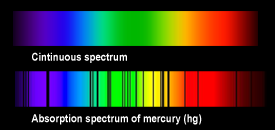
\includegraphics[width=.7\textwidth]{HgSpec.png}
	\caption{Kvicksilver absorbtionsspectrum.\cite{astronoo}}
	\label{fig:hgspec}
\end{figure}

%\begin{figure}[h]
%	\centering
%	\begin{subfigure}[c]{0.63\textwidth}
%	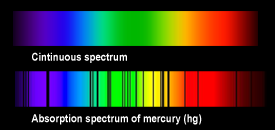
\includegraphics[width=\textwidth]{HgSpec.png}
%	\caption{Kvicksilver absorbtionsspectrum.\cite{astronoo}}
%	\label{fig:hgspec}
%	\end{subfigure}
%	~
%	\begin{subfigure}[c]{0.32\textwidth}
%	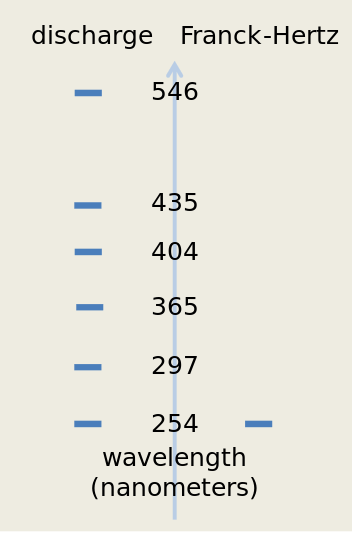
\includegraphics[width=\textwidth]{HgWavelen.png}
%	\caption{Take this picture away.}
%	\label{fig:hgwl}
%	\end{subfigure}
%	\caption{stuff}\label{fig:hgstuff}
%\end{figure}